\newcommand{\AtlasCoordFootnote}{ATLAS uses a right-handed coordinate system with its origin at the nominal interaction point
in the centre of the detector and the \(z\)-axis along the beam pipe.
The \(x\)-axis points from the interaction point to the centre of the LHC ring,
and the \(y\)-axis points upwards.
Cylindrical coordinates \((r,\phi)\) are used in the transverse plane, 
\(\phi\) being the azimuthal angle around the \(z\)-axis.
The pseudorapidity is defined in terms of the polar angle \(\theta\) as \(\eta = -\ln \tan(\theta/2)\).
Angular distance is measured in units of \(\Delta R \equiv \sqrt{(\Delta\eta)^{2} + (\Delta\phi)^{2}}\).}

%-------------------------------------------------------------------------------
\section{Overview}
%-------------------------------------------------------------------------------

%%% default ATLAS stuff

The ATLAS detector~\cite{PERF-2007-01} at the LHC covers nearly the entire solid angle around the collision point.\footnote{\AtlasCoordFootnote}
It consists of an inner tracking detector surrounded by a thin superconducting solenoid, electromagnetic and hadronic calorimeters,
and a muon spectrometer incorporating three large superconducting toroidal magnets.
The inner detector system (ID) is immersed in a \SI{2}{\tesla} axial magnetic field 
and provides charged-particle tracking in the range \(|\eta| < 2.5\).
The high-granularity silicon pixel detector covers the vertex region and typically provides four measurements per track, 
the first hit being normally in the insertable B-layer (IBL) installed before Run~2~\cite{ATLAS-TDR-2010-19,PIX-2018-001}.
It is followed by the silicon microstrip tracker (SCT) which usually provides eight measurements per track.
These silicon detectors are complemented by the transition radiation tracker (TRT),
which enables radially extended track reconstruction up to \(|\eta| = 2.0\).\footnote{Text taken from the ATLAS approved detectors text section of the repo, but I'm just including the tracker info since I use hits as my variables.} 
%%% end of default ATLAS stuff

A cutaway view of the ATLAS detector is shown in \Fig{ATLAS-detector}.  The inner detector (ID) provides charged particle tracking information closer to the interaction point.  The inner detector is immersed in a 2~T solenoidal magnetic field to bend the trajectories of charged particles and allow for momentum measurement. 
\begin{figure}[h!tbp]
\centering
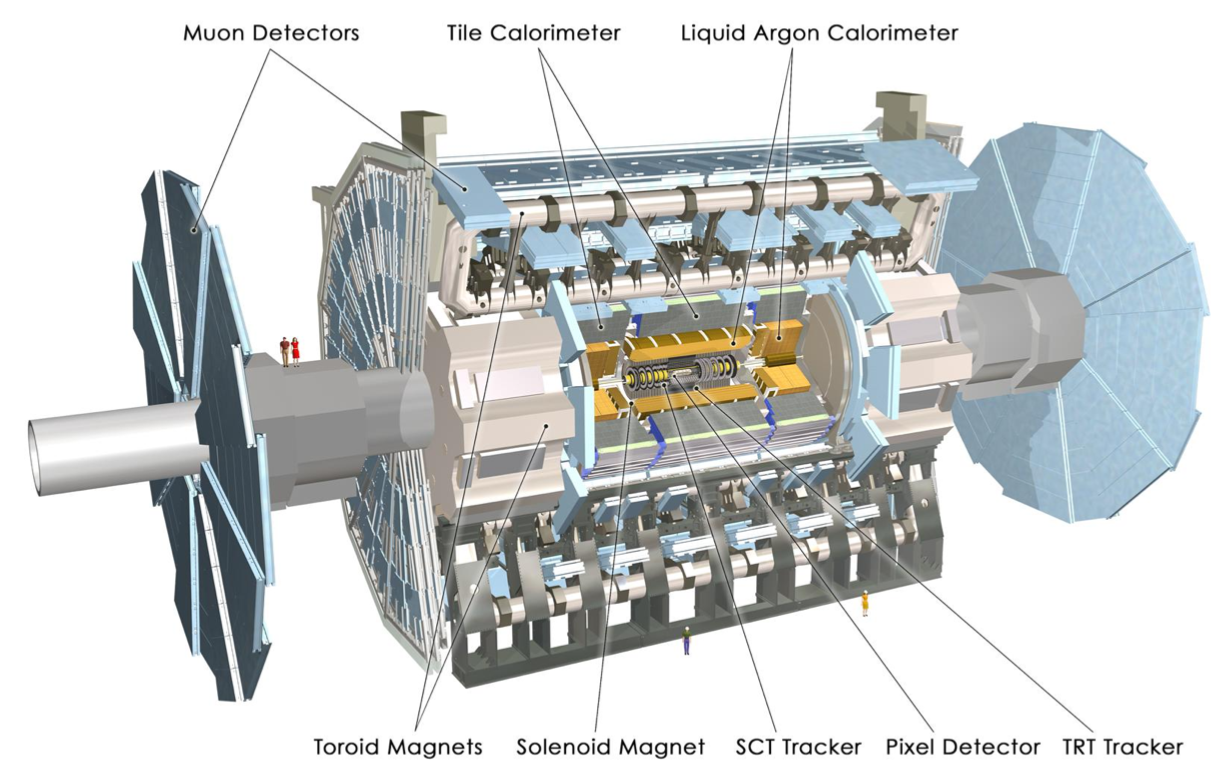
\includegraphics[width = \textwidth]{{\figpath/ATLAS_detector.png}}
\caption{Cut away of the ATLAS detector
~\cite{ATLAS_long}}
\label{ATLAS-detector}
\end{figure}
Energy measurement is made in two parts: with an electromagnetic and hadronic calorimeter.  Finally, the outermost layer of the detector is the muon spectrometer, with a 4~T toroidal magnetic field. 

\subsection{ATLAS Coordinate System}

At the ATLAS detector, the z-axis is measured along the accelerator beam pipe, the x-axis points into the center of the ring, and y-axis is defined to point vertically up by the properties of a right-handed rectilinear coordinate system.  
Then a cylindrical coordinate system is used for the ATLAS detector.
The azimuthal angle, $\phi = \arctan(\frac{y}{x})$, denotes orientation in the plane transverse to the beam, and the pseudorapidity, $\eta$, measures the polar angle inside the detector, where
%
\begin{equation}
\eta = -\ln \left( \tan \left(\frac{\theta}{2} \right) \right)
\end{equation}
%
and where $\theta \in [0,\pi]$ is the polar angle as measured from the z-axis.  The ATLAS detector is forward-backward symmetric to maximize the detector coverage since colliding protons each have the same energy.

From these detector variables, we can get components in the four-momentum using the relations %(derivation shown in Ref~\cite{eta_phi_Cartesian}).
\begin{equation}
(E,p_x, p_y, p_z) = (E,p_T \cos \phi, p_T \sin \phi,p_T \sinh \eta)
\label{momentum-conversion1}
\end{equation}
\begin{equation}
p = p_T \cosh \eta
\label{momentum-conversion2}
\end{equation}
We can also get a measurement of the momentum in the calorimeter for relativistic particles.  In the relativistic limit, the energy and momentum are the same (in natural units).  However, when the momentum is defined from a calorimeter measurement, $E_T$ is used instead of $p_T$. Equations~\eqref{momentum-conversion1} and \eqref{momentum-conversion2} still apply in this case.
